\label{sec:basdp}
We propose an approximate HMDP planner based on Symbolic Dynamic Programming that uses the XADD data structure and its efficient approximation to solve problems that couldn't solved exactly. We begin by formalizing a Hybrid MDP.

\subsection{Hybrid Markov Decision Processes (HMDPs) }
In HMDPs, states are represented by variable assignments. We assume a vectors of variables
$(\vec{b},\vec{x}) = ( b_1,\ldots,b_n,x_{1},\ldots,x_m )$, where each $b_i \in \{ 0,1 \}$ ($1 \leq i \leq n$) is boolean$\,$ and each $x_j \in \mathbb{R}$ ($1 \leq j \leq m$) is continuous. We also assume a finite set of $p$ parametrized actions $A = \{ a_1(\vec{y}_1), \ldots, a_p(\vec{y}_p) \}$, where $\vec{y}_k \in \mathbb{R}^{|\vec{y}_k|}$ ($1 \leq k \leq p$) denote continuous parameters for action $a_k$.

A HMDP model also requires the following: (i) a joint state transition model
$P(\vec{b}',\vec{x}'|\cdots,a,\vec{y})$, which specifies the
probability of the next state $(\vec{b}',\vec{x}')$ conditioned on a
subset of the previous and next state and action $a(\vec{y})$; (ii) a
reward function $R(\vec{b},\vec{x},a,\vec{y},\vec{b}',\vec{x}')$, which specifies the
immediate reward obtained by taking action $a(\vec{y})$ in state
$(\vec{b},\vec{x})$ and reaching state $(\vec{b}',\vec{x}')$; and (iii) a discount factor $\gamma, \; 0 \leq \gamma \leq 1$.

A policy $\pi$ specifies the action $a(\vec{y}) =
\pi(\vec{b},\vec{x})$ to take in each state $(\vec{b},\vec{x})$.  Our
goal is to find an optimal sequence of finite horizon-dependent
policies $\Pi^* = (\pi^{*,1},\ldots,\pi^{*,H})$ that
maximizes the expected sum of discounted rewards over a horizon $h \in
H; H \geq 0$:

\begin{align}
V^{\Pi^*}(\vec{b},\vec{x}) & = E_{\Pi^*} \left[ \sum_{h=0}^{H} \gamma^h \cdot r^h \Big| (\vec{b}_0,\vec{x}_0) \right]. \label{eq:vfun_def}
\end{align}
Here $r^h$ is the reward obtained at horizon $h$ following $\Pi^*$ where 
we assume starting state $(\vec{b}_0,\vec{x}_0)$ at $h=0$.
 
HMDPs as defined above are naturally factored~\cite{boutilier99dt}
in terms of state variables $(\vec{b},\vec{x})$; as such,
transition structure can be exploited in the form of a dynamic Bayes
net (DBN)~\cite{dbn} where the conditional probabilities
$P(b_i'|\cdots)$ and $P(x_j'|\cdots)$ for each next state variable can
condition on the action, current and next state.  We allow  
\emph{synchronic arcs} (variables that condition on each
other in the same time slice) between any pair of variables, binary $\vec{b}$ or
continuous $\vec{x}$, but we do not allow cyclic synchronic dependencies. 
The absence of synchronic cycles means there is a topological sorting of the variables according to the dependency graph implied by the model $P$: $\vec{v}_{sort}=topological\_sort_{P}( b_1,\ldots,b_n,x_{1},\ldots,x_m ) =  ( v_1,\ldots, v_{n+m})$, such that $v_k$ is independent of $v_j$, for all $j >k$. Hence we can factorize the joint transition model as
{\footnotesize
\begin{equation}
P(\vec{b}',\vec{x}'|\vec{b},\vec{x},a,\vec{y}) = 
\prod_{k=1}^{n+m} P(v_k'| \vec{b},\vec{x}, \vec{v}'_{<k}, a,\vec{y}) \nonumber %\label{eq:dbn} 
\end{equation}}
where $\vec{v}'_{<k} = ( v'_1,\ldots, v'_{k-1}), 1\leq k \leq n+m$

TODO: Illustrate MDP,DBN, with variable ordering fig~\ref{fig:hmdp}?

\begin{figure}[h!t]
\center
\fbox{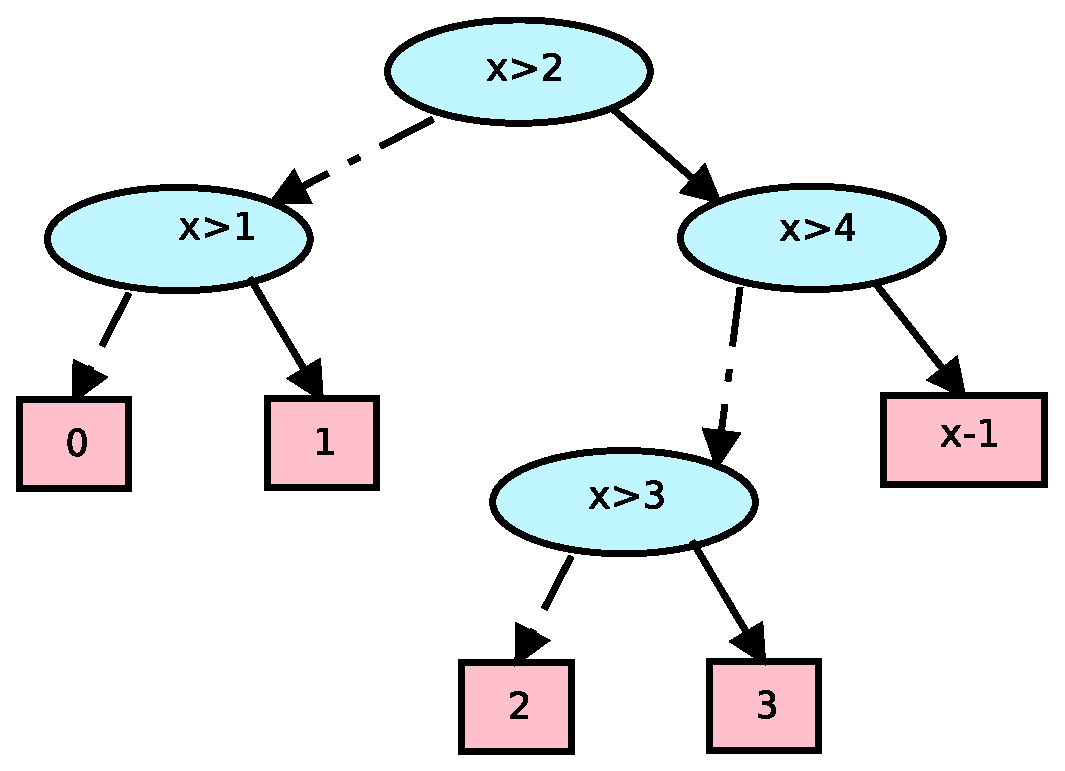
\includegraphics[scale=0.4]{Figures/xadds/samplexadd.eps} }
\caption{ Example of HMDP dynamic.}
\label{fig:hmdp} 
\end{figure}

The conditional probabilities functions $P(b_i'=v_{k_i}'|\vec{b},\vec{x},\vec{v}'_{<{k_i}},a,\vec{y})$ for \emph{binary} variables $b_i$ ($1 \leq i \leq n$) can condition on state and action variables.  

For the \emph{continuous} variables $x_j$ ($1 \leq j \leq m$), we represent the CPFs $P(x_j'=v_{k_j}'|\vec{b},\vec{x},\vec{v}'_{<{k_j}},a,\vec{y})$ with \emph{piecewise
linear equations} (PLEs) satisfying three properties: (i) PLEs 
can only condition on the action, current state, and previous state variables, (ii) PLEs are
deterministic meaning that to be represented by probabilities they
must be encoded using Dirac $\delta[\cdot]$ functions and (iii) PLEs are piecewise linear, where the piecewise conditions may be arbitrary logical combinations of the binary variables
and linear inequalities over the continuous variables. In more intuitive
terms, one can see that this $\delta[\cdot]$ is a simple way to encode
the PLE transition $x' = \left\{ \ldots \right.$ in the form of 
$P(x_j'=v_{k_j}'|\vec{b},\vec{x},\vec{v}'_{<{k_j}},a,\vec{y})$.

While it is clear that our restrictions do not permit general stochastic transition
noise (e.g., Gaussian noise as in LQG control), they do permit
discrete noise in the sense that $P(x_j'=v_{k_j}'|\vec{b},\vec{x},\vec{v}'_{<{k_j}},a,\vec{y})$ may condition on $\vec{b'}$, which are stochastically sampled according to their CPFs.
We note that this representation effectively allows modeling of
continuous variable transitions as a mixture of $\delta$ functions,
which has been used frequently in previous exact continuous state MDP
solutions~\cite{feng04,hao09}.

% TODO: Not li05 here (allowed PWC probability), another?

We allow the reward function $R(\vec{b},\vec{x},a,\vec{y},\vec{b}',\vec{x}')$ to be
a general piecewise linear function (boolean or linear conditions
and linear values) such as
\begin{align}
R(\vec{b},\vec{x},a,\vec{y},\vec{b}',\vec{x}') = \begin{cases}
b \land x_1 \leq x_2 + 1 : & 1 - x_1' + 2x_2' \\
\neg b \lor x_1 > x_2 + 1:     & 3x_1 + 2x_2 \\
\end{cases} \label{eq:linear_reward}
\end{align}

These transition and reward constraints ensure that all derived
functions in the solution of these hybrid MDPs will remain piecewise linear, which 
is essential for our approximation and efficient representation.

\subsection{Solution Methods}

\label{sec:soln}

The algorithm we use for solving HMDPs, is an approximate version of the continuous state and action generalization of {\it value iteration}~\cite{bellman}, which is a dynamic programming algorithm for constructing optimal policies.  It proceeds by constructing a series of $h$-stage-to-go optimal value functions $V^h(\vec{b},\vec{x})$.
Initializing $V^0(\vec{b},\vec{x}) = 0$) we define the quality
$Q_a^{h}(\vec{b},\vec{x},\vec{y})$ of taking action $a(\vec{y})$ in state
$(\vec{b},\vec{x})$ and acting so as to obtain $V^{h-1}(\vec{b},\vec{x})$ thereafter as the following:
\vspace{-2.5mm}
{\footnotesize
\begin{align}
& Q_a^{h}(\vec{b},\vec{x},\vec{y}) = \sum_{\vec{b}'} \hspace{-1.0mm} \int_{\vec{x}'} \hspace{-1.0mm} \Bigg[ R(\vec{b},\vec{x},a,\vec{y},\vec{b}',\vec{x}') +  \label{eq:qfun} \\ 
& \gamma \cdot \left( \prod_{k=1}^{n+m} P(v_k'| \vec{b},\vec{x}, \vec{v}'_{<k}, a,\vec{y}) V^{h-1}(\vec{b}',\vec{x}') d\vec{x}' \right)  \Bigg] \nonumber
\end{align}}
Given $Q_a^h(\vec{b},\vec{x})$ for each $a \in A$, we can proceed
to define the $h$-stage-to-go value function as follows:
\begin{align}
V^{h}(\vec{b},\vec{x}) & = \max_{a \in A} \max_{\vec{y} \in \mathbb{R}^{|\vec{y}|}} \left\{ Q^{h}_a(\vec{b},\vec{x},\vec{y}) \right\} \label{eq:vfun}
\end{align}

If the horizon $H$ is finite, then the optimal value function is
obtained by computing $V^H(\vec{b},\vec{x})$ and the optimal
horizon-dependent policy $\pi^{*,h}$ at each stage $h$ can be easily
determined via $\pi^{*,h}(\vec{b},\vec{x}) = \argmax_{(a, \vec{y} )} Q^h_a(\vec{b},\vec{x},\vec{y})$.  If the horizon $H
= \infty$ and the optimal policy has finitely bounded value, then
value iteration can terminate at horizon $h$ if $V^{h} = V^{h-1}$;
then $V^\infty = V^h$ and $\pi^{*,\infty} = \pi^{*,h}$.

Here we show the code of the SDP algorithm, Alg.~\ref{alg:vi}. The function Regress computes the result of equation~\ref{eq:qfun}, we note that all the operations involved, namely multiplication, integration of continuous $\delta$ functions and marginalization of boolean variables, are defined XADDs. Due to lack of space, its implementation is omitted and we refer to \cite{zamani12} for a precise description of these operations.

\incmargin{.5em}
\linesnumbered
\begin{algorithm}[th!]
\vspace{-.5mm}
\dontprintsemicolon
\SetKwFunction{regress}{Regress}
\SetKwFunction{approximate}{Approximate}
\Begin{
   $V^0:=0, h:=0$\;
   \While{$h < H$}{
       $h:=h+1$\;
       \ForEach {$a(\vec{y}) \in A$}{
              $Q_a^{h}(\vec{y})\,:=\,$\regress{$V^{h-1},a,\vec{y}$}\;
              $Q_a^{h} := \max_{\vec{y}} \, Q_a^{h}(\vec{y})$ $\,$ \emph{// Continuous $\max$}\;
              $V^{h} := \casemax_a \, Q_a^{h}$ $\,$ \emph{// $\casemax$ all $Q_a$}\;
              $\pi^{*,h} := \argmax_{(a,\vec{y})} \, Q_a^{h}(\vec{y})$\;
       }
       $V^h = $\approximate{$V^{h}$}\; \label{approxline}
       \If{$V^h = V^{h-1}$}
           {break $\,$ \emph{// Terminate if early convergence}\;}
   }
     \Return{$(V^h,\pi^{*,h})$} \;
}
\caption{\footnotesize \texttt{VI}(Hybrid-MDP, $H$) $\longrightarrow$ $(V^h,\pi^{*,h})$ \label{alg:vi}}
\vspace{-1mm}
\end{algorithm}
\decmargin{.5em}


\subsection{Bounded Approximate SPD}
We will now properly define the Hybrid MDP planing algorithm described in this paper. The SDP algorithm~\ref{alg:vi} was modified from its original exact version by the addition of line \ref{approxline} which uses the algorithm~\ref{alg:approx}, responsible for collecting the cases and making the global approximation by combining the successive pairwise merges.

